\RequirePackage{luatex85}
\documentclass[tikz]{standalone}
% Default preamble
\usepackage{pgfplots}
\pgfplotsset{compat=newest}
\usepgfplotslibrary{groupplots}
\usepgfplotslibrary{polar}
\usepgfplotslibrary{smithchart}
\usepgfplotslibrary{statistics}
\usepgfplotslibrary{dateplot}
\usepgfplotslibrary{ternary}
\usepackage[T1]{fontenc}
\usepackage{lmodern}
\begin{document}
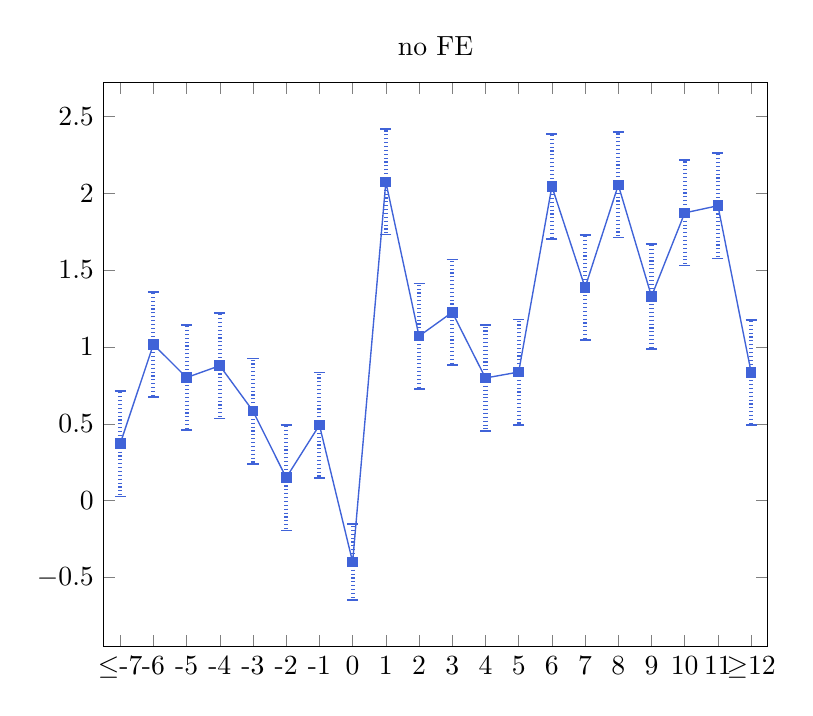
\begin{tikzpicture}
\begin{axis}[title={no FE}, title style={}, xlabel style={}, ylabel style={}, xticklabel style={}, yticklabel style={}, width={240pt}, height={204pt}, symbolic x coords={$\leq$-7,-6,-5,-4,-3,-2,-1,0,1,2,3,4,5,6,7,8,9,10,11,$\geq$12}, xtick={$\leq$-7,-6,-5,-4,-3,-2,-1,0,1,2,3,4,5,6,7,8,9,10,11,$\geq$12}, xmin={{[normalized]-0.5}}, xmax={{[normalized]19.5}}, scale only axis]
    \addplot[mark={square*}, mark options={mark size={1.75pt}, line width={0pt}, fill={rgb,255: red, 64; green, 99; blue, 216}, fill opacity={1}, draw={rgb,255: red, 64; green, 99; blue, 216}, draw opacity={1}}, error bars/error mark={|}, error bars/error mark options={mark size={2.0pt}, solid, line width={0.6pt}, fill={rgb,255: red, 64; green, 99; blue, 216}, fill opacity={1}, draw={rgb,255: red, 64; green, 99; blue, 216}, draw opacity={1}}, error bars/error bar style={draw={rgb,255: red, 64; green, 99; blue, 216}, draw opacity={1}, densely dotted, line width={1.5pt}}, draw={rgb,255: red, 64; green, 99; blue, 216}, draw opacity={1}, line width={0.5pt}, error bars/y dir={both}, error bars/y explicit]
        coordinates {
            ($\leq$-7,0.36968848040224606) +- (0,0.34266703123023107)
            (-6,1.0161642543359548) +- (0,0.3426670312302312)
            (-5,0.8004351374649953) +- (0,0.34266703123023107)
            (-4,0.8778993522840777) +- (0,0.34266703123023107)
            (-3,0.5827695112478852) +- (0,0.3426670312302312)
            (-2,0.14944225350724588) +- (0,0.34266703123023107)
            (-1,0.49160731110002853) +- (0,0.342667031230231)
            (0,-0.398469527810116) +- (0,0.24536538956165185)
            (1,2.072646366698694) +- (0,0.3426670312302311)
            (2,1.0699196982728512) +- (0,0.3426670312302311)
            (3,1.2250710642968228) +- (0,0.34266703123023107)
            (4,0.797671985702105) +- (0,0.34266703123023107)
            (5,0.8364708751691294) +- (0,0.34266703123023107)
            (6,2.043744880797379) +- (0,0.34266703123023107)
            (7,1.3859074708972914) +- (0,0.34266703123023107)
            (8,2.052924230676941) +- (0,0.34266703123023107)
            (9,1.3283311252365624) +- (0,0.342667031230231)
            (10,1.8713616815794538) +- (0,0.34266703123023107)
            (11,1.9179877639249492) +- (0,0.34266703123023107)
            ($\geq$12,0.8338398361407305) +- (0,0.34266703123023107)
        }
        ;
\end{axis}
\end{tikzpicture}
\end{document}
